\documentclass{llncs}

\usepackage{url}
\usepackage{graphicx}
\usepackage{listings}
\usepackage{verbatim}
\usepackage[lined,linesnumbered,algochapter]{algorithm2e}
\usepackage{tikz}
\usetikzlibrary{arrows,automata}
\usepackage{xspace}
\usepackage{todonotes}          % Package for working draft comments


\usepackage[english]{babel}

\setcounter{secnumdepth}{2}
\setcounter{tocdepth}{3}

% define custom macros for specific formats or names
\newcommand{\uml}[1]{\texttt{#1}}
\newcommand{\cd}{\textsf{Class Diagram}}

\begin{document}
\pagestyle{plain}
\pagenumbering{roman}

\title{fUML Refactoring with EMF\footnote{This work has been created in the context of the course ``Advanced Model Engineering'' (188.952) in SS14.}}

\author{Sebastian Geiger (1127054) \and Kristof Meixner (9725208)}
\institute{Business Informatics Group\\Vienna Technical University}

\maketitle

\begin{abstract}
In this work we will present some ideas and concepts for the refactoring of fUML. The main contribution of this work is the extension of
existing UML refactorings to cover not only the static aspect of UML such as class diagrams but to also include refactorings for dynamic
parts such as activity diagrams. In this work we will present basic concepts for refactoring with EMF and show how model semantics can be
preserved through the use of OCL constraints. In the remainder of the paper we then present our tool chain and the used technologies
such as EMF and Ecore and how we used them for refactoring. We also present a discussion of EMF.Refactor, which shows how such refactorings
can be made available in the Eclipse GUIs such as the EMF tree editor or Papyrus.
\end{abstract}

\tableofcontents
\newpage

\pagenumbering{arabic}

\section{Introduction}
The concept of refactoring is an important part of software development which should be included in every cycle of iterative and evolutionary
software development. It main goal is to reorganise software components to achieve better design, lower coupling, higher cohesion, and other
attributes which make up good software design. The important aspect of refactoring is that no additional features are introduced during
a refactoring step and the semantics of the software are maintained; no additional bugs or errors are introduced. Refactoring can not only
be applied to source code but as well to models such as UML or fUML models. In the context of models such as class diagrams, it means that
the structure of the diagram is rearranged to achieve a better design. This included changing superclass releationships, moving attributes
and methods to different classes or adding new interfaced. A catalogue of possible UML refactorings can be found in \todo{cite markovic}.

fUML is an extension of UML which builds on a subset of UML classes with the purpose of adding semantics to UML models such that they can
be executed on the model level. The dominant concept for this is the activity diagram. If a refactoring is performed on a UML model such
as a class diagram, then any activity diagram which is releated to the class diagram, has to be checked and possibly changed as well. In
section \ref{sec:fuml-refactoring} we will present some examples of fUML activity diagrams and present the implications that result from
changing class diagrams.

Since a refactoring changes the structure of a model it is important to ensure that all changes maintain the original semantics of the
model. Violating this requirement can result in models with either a different behavior, or in models which can no longer be executed.
To ensure semantic preservation, two main techniques can be used. First, the refactoring can be broken down into smaller steps, each of
which either guarantees to preseve the semantics of the model or makes it easier to verify that this is the case. Second, logical
constraints can be used to limit refactorings on models to only those cases where semantic preservation can be ensured. For this
purpose pre- and postconditions are specified with OCL constraints. A refactoring is then only applied if the original model satisfies
the precondition before the refactoring is applied and the postcondition after the refactoring has been completed. Such constrains must
be individually specified for each kind of refactoring that is to be performed, as such a part of this paper will discuss different OCL
constraints for the refactorings that we introduce.

% what is refactoring and what does it mean in the context of models?
% what is fuml? what does fuml consist for diagram types?
% what is ocl? why do we use it and what for?

%fUML adds semantics to UML models that make it possible to create semantically closed models which can be executed on the model level. With
%fUML classic refactorings are not enough to refactor those models as they do not support the refactoring of the dynamic aspects of models
%such as activity diagrams.

\section{Motivation}
% what do we want to achieve?

In this paper we will present a set of refactorings and give examples of how each refactoring can be applied to a concrete model. 

% Why is it interesting to refactor models
% Why is it important in fUML that models remain consistent -> to preserve executability
% It is possible to use pre and post conditions in OCL to guarantee the semantic preservation of models during refactorings.

\section{Refactorings Examples}
% take model refactorings of markovic paper
% insurance example
% create example that supports all proposed refactorings

This section covers some general refactorings of UML class diagrams. As the basis of these refactorings an example from the insurance
domain is used. In the insurance business there are domain objects such as an insurance policy. Cars and trucks can be insured by 
adding them to the policy. There is an insurance company which has customers and employees and employees may purchase an insurance policy 
for one of their cars or trucks. Figure \ref{fig:classdiagramcomplex} shows a class diagram of such an insurance policy. This class 
diagram would benefit from several possible refactorings such as an \textit{extract superclass} which can be applied to both Car and Truck 
to extract a Vehicle class. A simple \textit{extract class} can be used on InsurancePolicy to extract the from and until dates into their
own InsurancePeriod class. As part of the \textit{extract superclass} refactoring two additional refactorings namely \textit{pull up 
attribute} and \textit{pull up method} are used to move the identical attributes and methods of both classes to the new superclass. As the 
attributes weight and registration are public, we can use \textit{encapsulate field} to make them private and provide getter and setter 
implementations. Finally the method addCar can be renamed into addVehicle with \textit{rename method} and the addTruck method can be 
removed with \textit{remove method}.

\begin{figure}[h!t]
 \centering
 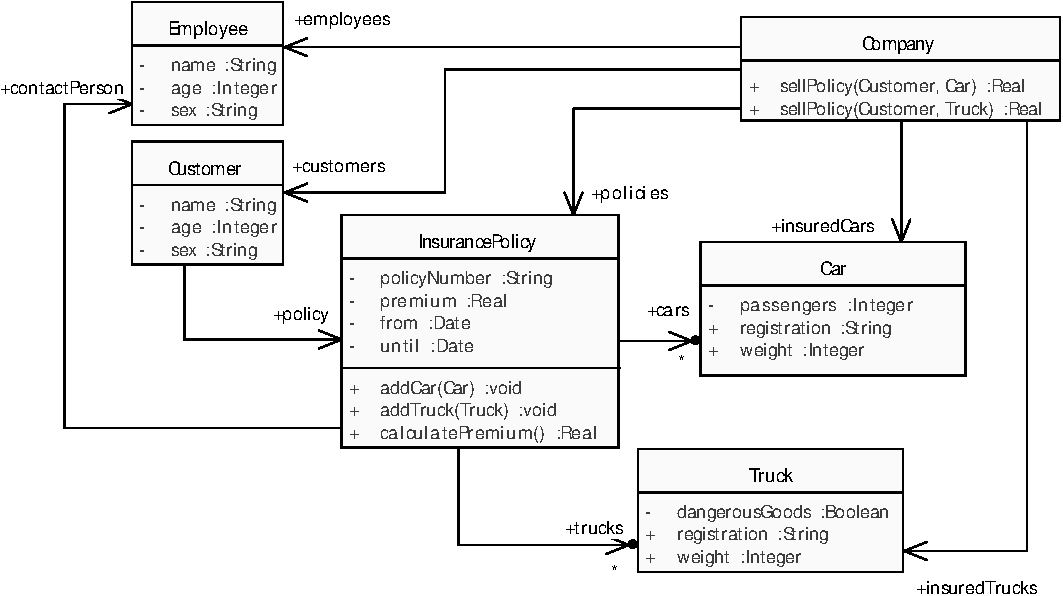
\includegraphics[scale=0.7]{images/ClassDiagramComplex.pdf}
 \caption{A car object that could benefit of extract class}
 \label{fig:classdiagramcomplex}
\end{figure}

For each of the methods the \textit{InsurancePolicy} and \textit{Company} classes a separate activity diagram exists which defines the
semantics of these methods. As some of them are quite similar we will present only the diagrams for addCar(), sellPolicy(Customer, Car) and calculatePremium().






Figure \ref{fig:complexcar} shows an example of a more complex car object which captures additinoal information about the owner which is allowed to drive the car. This example would benefit from an \textit{extract class} refactoring. The extract class refactoring would pull the members 
The policy allows to insure cars and trucks. Both Car and Truck have some attributes that are similar (weight, registration) and others that
are different (dangerousGoods, passengers). From the 

\begin{figure}[ht]
 \centering
 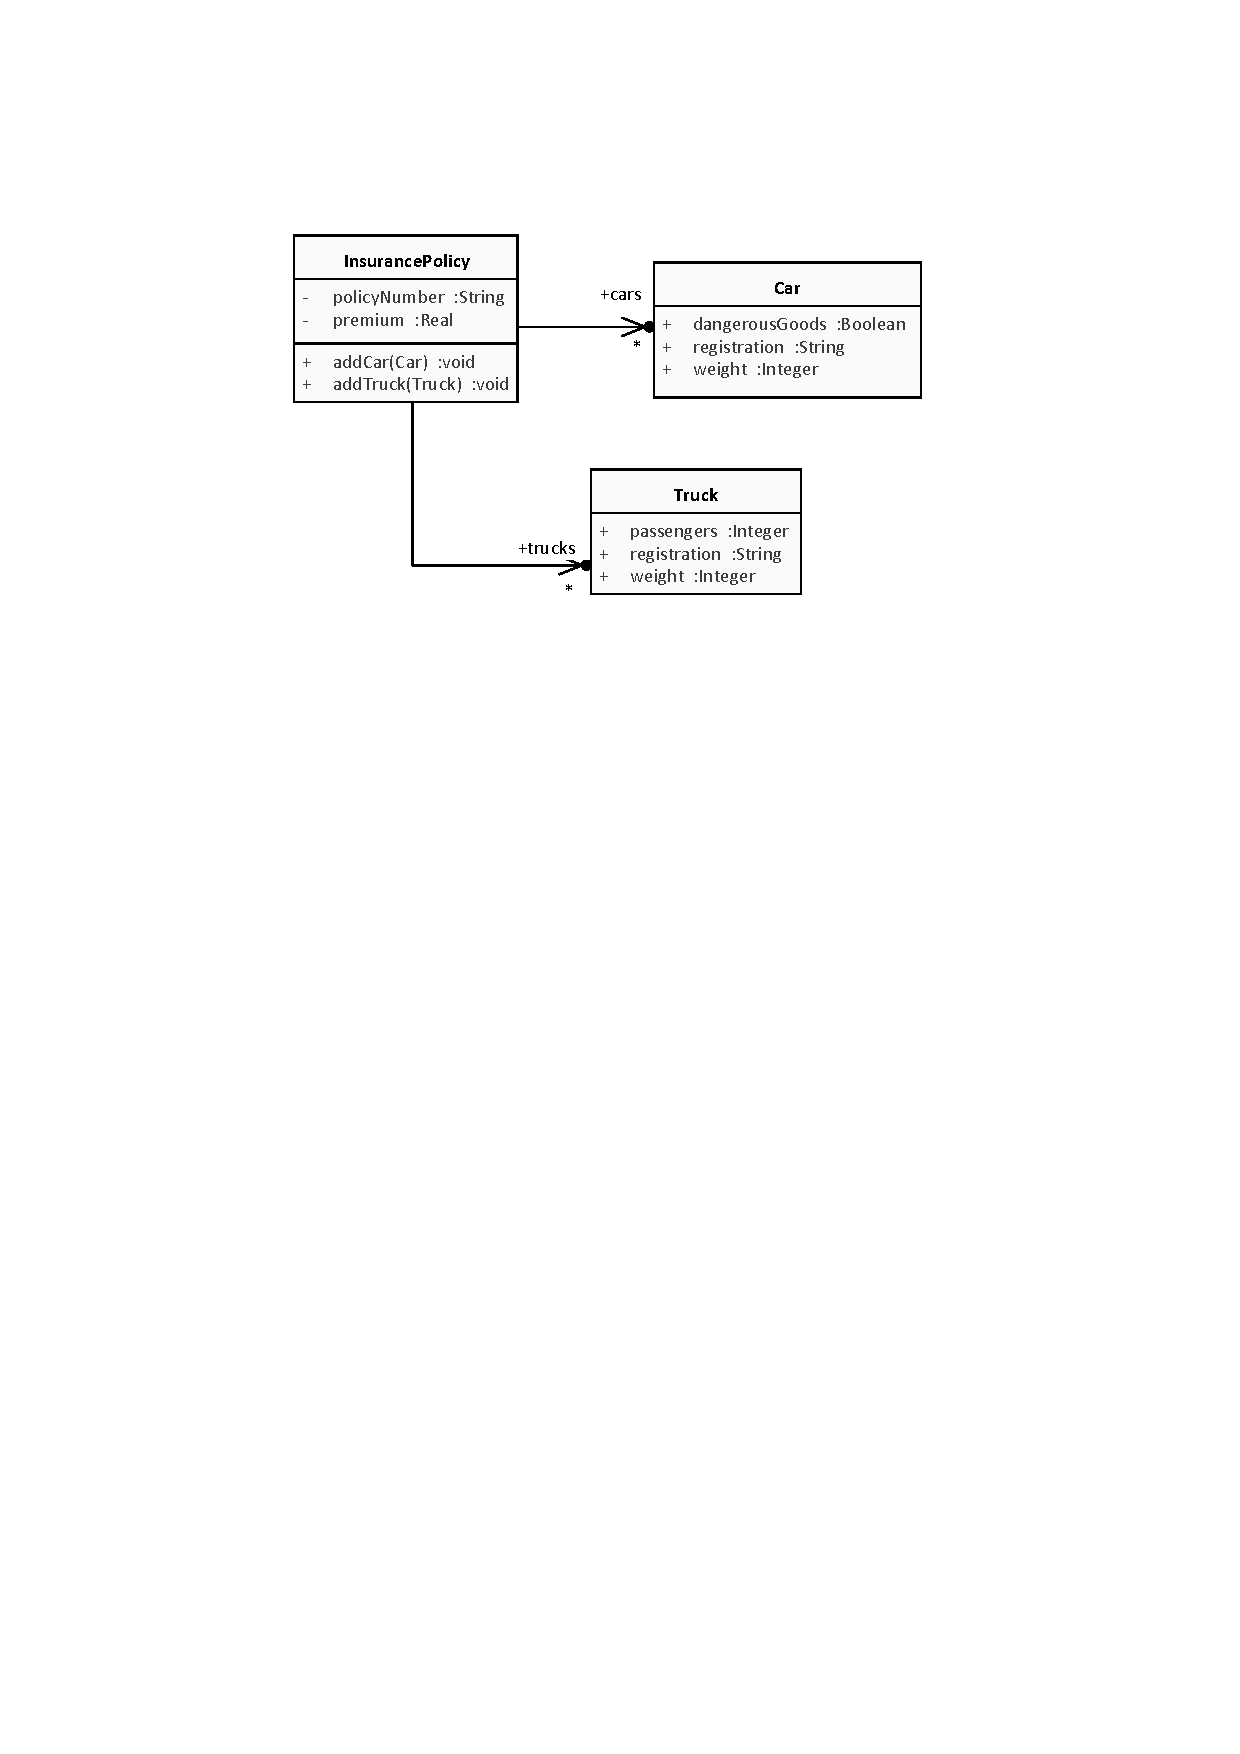
\includegraphics{images/addCar-class_diagram.pdf}
 \caption{Insurance policy class diagram}
 \label{fig:insurancepolicy}
\end{figure}

\begin{figure}
 \centering
 \begin{tabular}[]{l}
  \hline
  Extract class\\
  Extract superclass\\
  Rename Class\\
  Rename Method\\
  Rename Variable\\
  Add / Remove Parameter\\
  Encapsulate Field\\
  Pull up attribute\\
  Pull up operation\\
  Pull up association end\\
  Remove unused class\\
  \hline
 \end{tabular}
 \caption{Refactoring examples}
 \label{fig:refactoringlist}
\end{figure}

In this section we will present some general refactorings such as the ``extract superclass'' refactoring. A list of example refactorings
is presented in figure \ref{fig:refactoringlist}.




\begin{figure}[ht]
 \centering
 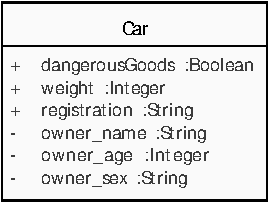
\includegraphics{images/ComplexCar-class_diagram.pdf}
 \caption{A car object that could benefit of extract class}
 \label{fig:complexcar}
\end{figure}


\section{Refactoring of fUML diagrams}
\label{sec:fuml-refactoring}
% abstract syntax of fUML and changes in diagrams
% ecore and ocl (with code examples)
In this section we will present some general refactorings

\begin{figure}[ht]
 \centering
 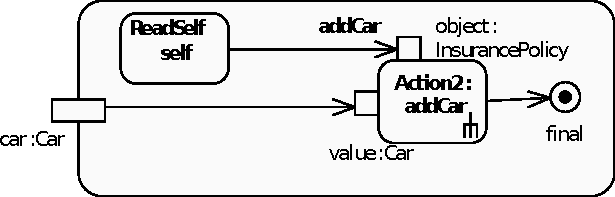
\includegraphics{images/addCar-activity_diagram}
\end{figure}

\section{Tool chain and implementation}
For our tool chain we have relied on the moliz\footnote{source...} repository, mainly for the ability to execute the fUML models with
a virtual machine. The models are stored as XMI 
% usage of fUML reference implementation of BIG
% how to load models?
% how to execute models?
% how to apply queries and changes?

\subsection{Model refactoring}
Describe our tool chain, how we created models, how we load them, what information of the abstract syntax we use for refactoring, etc.

\subsection{GUI Integration}
Describe what we did with EMF.Refactor.

\section{Related Works}
% papers we read
% what we did that they didnt
We have compared our works with several other available papers. In [..] there is a discussion of uml refactings which covers ....

some related works such as ... 

% we need at least one citation in the document or an error occurs. Remove this line after we have other citations in the document.
\cite{rob99}

\section{Conclusion}
We conclude this paper with...

\bibliographystyle{acm}
\bibliography{references}

\end{document}
